\section{Server}
The most important job of the server is to facilitate communication between clients.
It was therefore decided to make the server as simple as possible, just providing simple methods of storing and retrieving data from the database without performing any operations on the data.
While the server does not know anything about the data that is sent and received by clients, it is supposed to handle user authentication and authorization as described in section~\ref{sec:security}.
The various actions that can be performed on the server can be found in Appendix~1.

\subsection{Server architecture}
\begin{figure}[H]
\begin{center}
	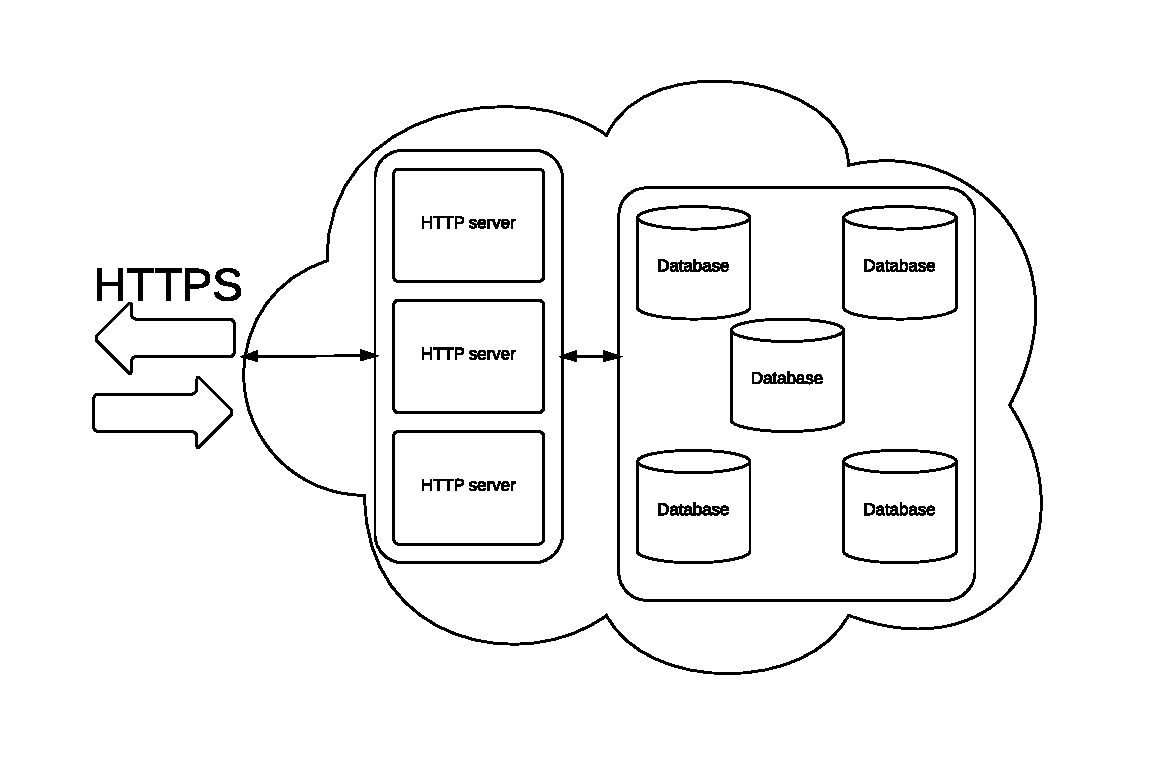
\includegraphics[scale=0.75]{graphics/server.pdf}
	\caption{The server architecture.}
	\label{fig:server-architecture}
\end{center}
\end{figure}
The most important piece of software utilized is the database, MongoDB\footnote{\url{https://www.mongodb.org/}}.
There were two main reasons for choosing MongoDB.
First: it is a schema-less database.
This means that we can simply send data to the database without first telling the database what the data looks like, that is what kind of data it is supposed to store (numbers, text, coordinates, etc.), and how much there is of it.
The second reason that MongoDB was chosen was because it is built to easily scale by adding more database servers.
This means that as more and more clients are added to the system, scaling can be done easily in an automated fashion by powering up more servers with exactly the same database software.

The web server responsible for handling communication between the software responsible for database communication and clients is nginx\footnote{\url{http://nginx.org/}}.
It is a modern web server built for handling a large amount of concurrent users on a single web server.

The web server communicates with the software we have written in the programming language Python, which then handles storing and retrieving data from the database.
Notes on how to set up the server can be found in the installation notes of Appendix~4.

\subsection{Further server development}
The first thing that should be implemented to get the server ready for production is implementing authentication and access restriction as described in section~\ref{sec:security}.
Security is very important, and also very hard, so it would be worth it to use at least as much time as we've had so far to develop and test the security measures.

Another thing that is important to add is a way to manage clients on the server.
Currently it is required to have direct access to the databases to add or remove clients.
The bare minimum required to get started would be a call for registering a client with a public key and a call for managing permissions to let other clients access the data of agents.

A new feature that is not strictly needed, but could provide helpful in extending the possibilities of the server is a way to help clients establish direct connections with each others.
Currently the server has great performance for sensor data where near real-time information is sent to a lot of user clients.
In order to be able to stream data (for example video and audio, but also other kinds of data) between clients right now it is required to use another service to set up the stream, just storing an identifier on the server.
Ideally, the server should be able to tell clients where they can find each order so that they can set up real-time streams directly.
